\tableofcontents
\section*{Предисловие}
При выполнении данной лабораторной работы было решено использовать 
\href{https://python-control.readthedocs.io/en/0.9.4/}{Python Control Systems Library}.
Данный инструмент является альтернативой Matlab, адаптированной для использования на 
языке Python и предоставляет широкий функционал для анализа и моделирования систем,
а также синтеза регуляторов для управления.

Полный листинг моделирования систем представлен в \href{https://github.com/diuzhevVlad/control-theory-itmo-fall-2023/blob/main/Lab5/Lab5.ipynb}{jupyter notebook} на GitHub.

\pagebreak

\section{Исследование типовых звеньев}
Рассмотрим несколько систем из приведенных заданий. Выведем дифференциальные уравнения, описывающие данные 
системы и найдем аналитические выражения для временных и частотных характеристик. Получение аналитических решений представленно
в листинге программы.
\subsection*{Brushed DC motor 2.0}
\begin{equation}
    J \dot{\omega} = M, M = k_m I, I = \frac{U+\varepsilon}{R}, \varepsilon = \varepsilon_i + \varepsilon_s, \varepsilon_i=-k_e \omega, \varepsilon_s=-L\dot{I}
\end{equation}
Путем преобразований можем получить дифференциальное уравнение (апериодическое звено второго порядка):
\begin{equation*}
    \ddot{\omega} + \frac{R}{L}\dot{\omega}+\frac{k_mk_e}{JL}\omega = \frac{k_m}{JL}U, W(s)=\frac{k_m}{JLs^2 + JRs + k_mk_e}
\end{equation*}
Временные характеристики:
\begin{equation*}
    y_{i.r.}=\mathcal{L}^{-1}(W(s)) = \frac{2 k_{m} e^{- \frac{R t}{2 L}} \sin{(\frac{t \sqrt{\frac{- \frac{R^{2}}{L} + \frac{4 k_{e} k_{m}}{J}}{L}}}{2} )} \theta(t)}{J L \sqrt{\frac{- \frac{R^{2}}{L} + \frac{4 k_{e} k_{m}}{J}}{L}}}
\end{equation*}
\begin{equation*}
    y_{s.r.}=\mathcal{L}^{-1}(\frac{1}{s}W(s)) = \frac{\theta(t)}{k_{e}} - \frac{e^{- \frac{R t}{2 L}} \cos{(\frac{t \sqrt{- R^{2} + \frac{4 L k_{e} k_{m}}{J}}}{2 L} )} \theta(t)}{k_{e}} - \frac{R e^{- \frac{R t}{2 L}} \sin{(\frac{t \sqrt{- \frac{R^{2}}{L^{2}} + \frac{4 k_{e} k_{m}}{J L}}}{2} )} \theta(t)}{L k_{e} \sqrt{- \frac{R^{2}}{L^{2}} + \frac{4 k_{e} k_{m}}{J L}}}
\end{equation*}
Проведем моделирование системы и сравним с аналитически полученным поведением:
\begin{figure}[h]
    \centering
    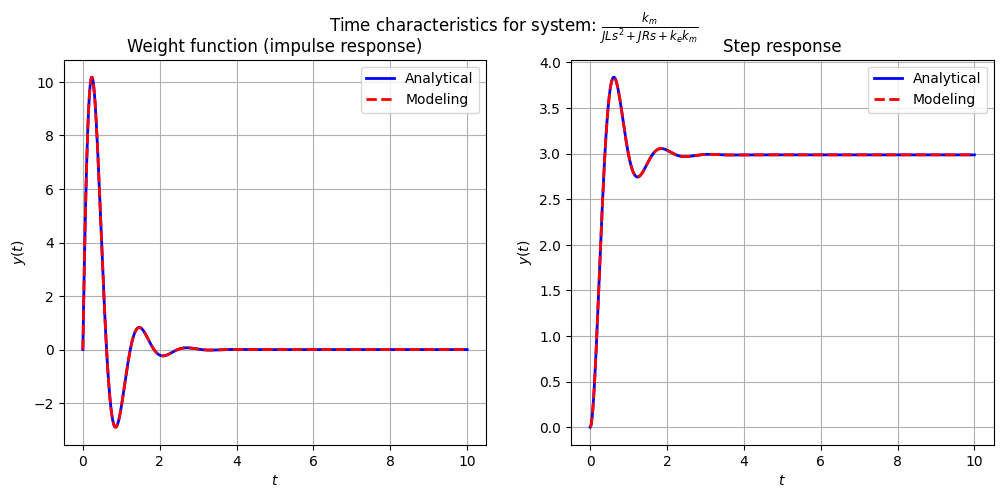
\includegraphics[width=\textwidth]{time_char_2.png}
    \caption{\label{fig:The-caption-1}Временные характеристики системы 2 (подвариант 7)}
\end{figure}

Частотные характеристики:
\begin{equation*}
    |W(j\omega)| = \frac{\|{k_{m}}\|}{\sqrt{J^{2} L^{2} \omega^{4} + J^{2} R^{2} \omega^{2} - 2 J L k_{e} k_{m} \omega^{2} + k_{e}^{2} k_{m}^{2}}}
\end{equation*}
\begin{equation*}
    Arg(W(j\omega)) = \operatorname{atan}_{2}{(- \frac{J R k_{m} \omega}{J^{2} R^{2} \omega^{2} + (J L \omega^{2} - k_{e} k_{m})^{2}},- \frac{k_{m} (J L \omega^{2} - k_{e} k_{m})}{J^{2} R^{2} \omega^{2} + (J L \omega^{2} - k_{e} k_{m})^{2}} )}
\end{equation*}
Воспользуемся функцией $\bold{bode}$ для численного моделирования частотных характеристик:
\begin{figure}[h]
    \centering
    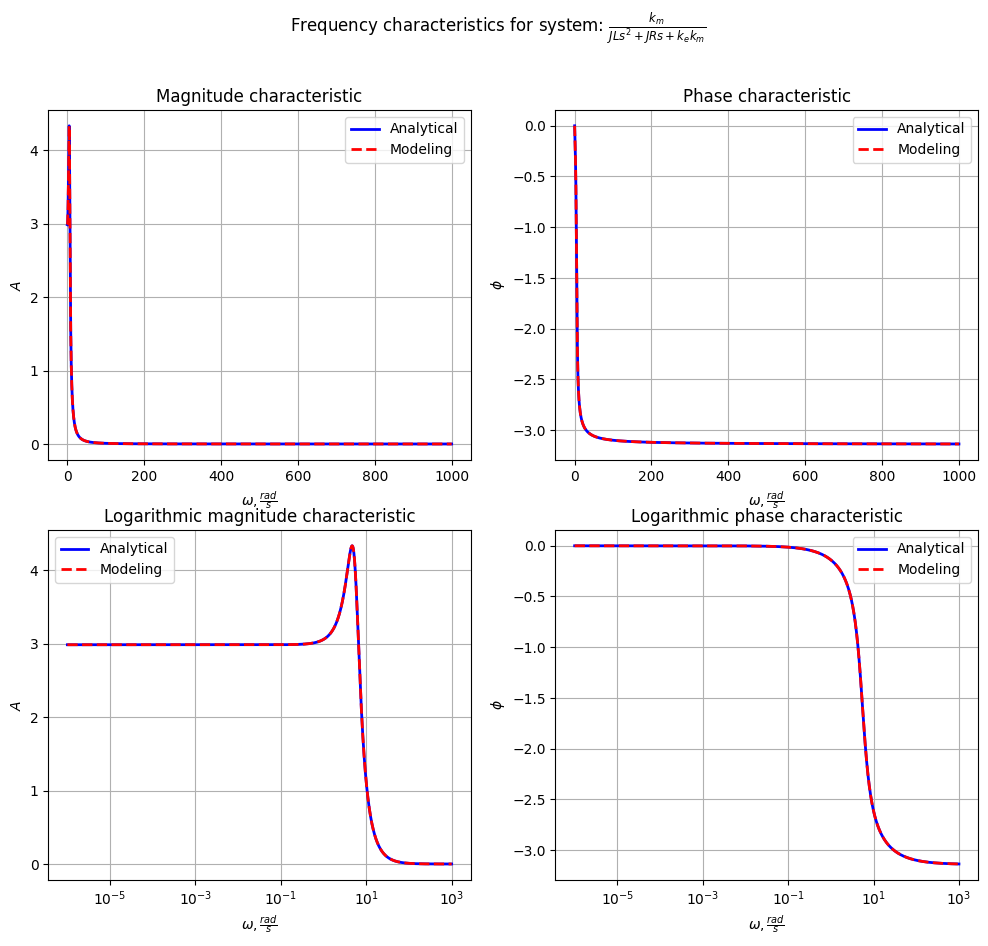
\includegraphics[width=\textwidth]{freq_char_2.png}
    \caption{\label{fig:The-caption-1}Частотные характеристики системы 2 (подвариант 7)}
\end{figure}
\pagebreak

\subsection*{Конденсируй. Интегрируй. Умножай}
\begin{equation}
    I = C\frac{dU}{dt}
\end{equation}
Путем преобразований можем получить дифференциальное уравнение (идеальное интегрирующее):
\begin{equation*}
    \dot{U}C = I, W(s)=\frac{1}{Cs}
\end{equation*}
Временные характеристики:
\begin{equation*}
    y_{i.r.}=\mathcal{L}^{-1}(W(s)) = \frac{\theta(t)}{C}
\end{equation*}
\begin{equation*}
    y_{s.r.}=\mathcal{L}^{-1}(\frac{1}{s}W(s)) = \frac{\theta(t)t}{C}
\end{equation*}
Проведем моделирование системы и сравним с аналитически полученным поведением:
\begin{figure}[h]
    \centering
    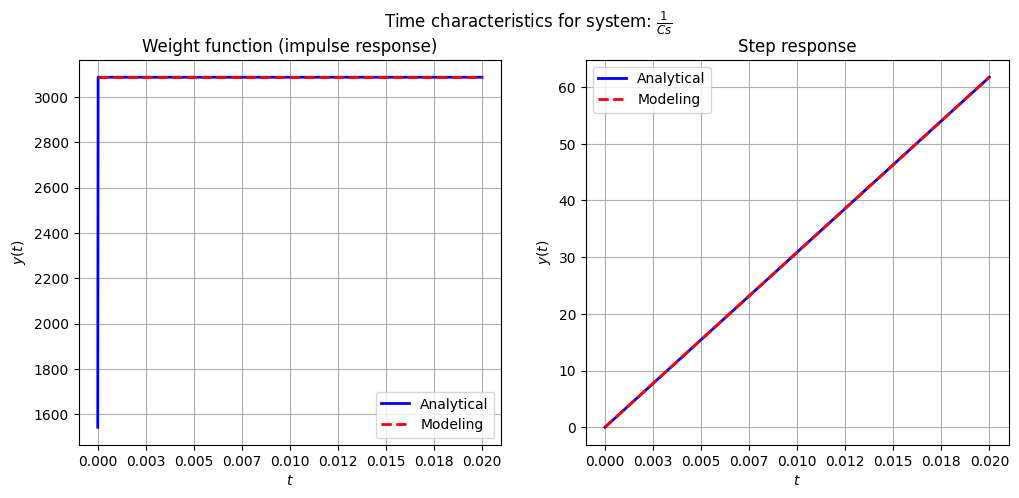
\includegraphics[width=\textwidth]{time_char_3.png}
    \caption{\label{fig:The-caption-1}Временные характеристики системы 3 (подвариант 7)}
\end{figure}

Частотные характеристики:
\begin{equation*}
    |W(j\omega)| = \frac{1}{|C\omega|}
\end{equation*}
\begin{equation*}
    Arg(W(j\omega)) = \operatorname{atan}_{2}{(-\frac{1}{C\omega},0)}=-\frac{\pi}{2}
\end{equation*}
Воспользуемся функцией $\bold{bode}$ для численного моделирования частотных характеристик:
\begin{figure}[]
    \centering
    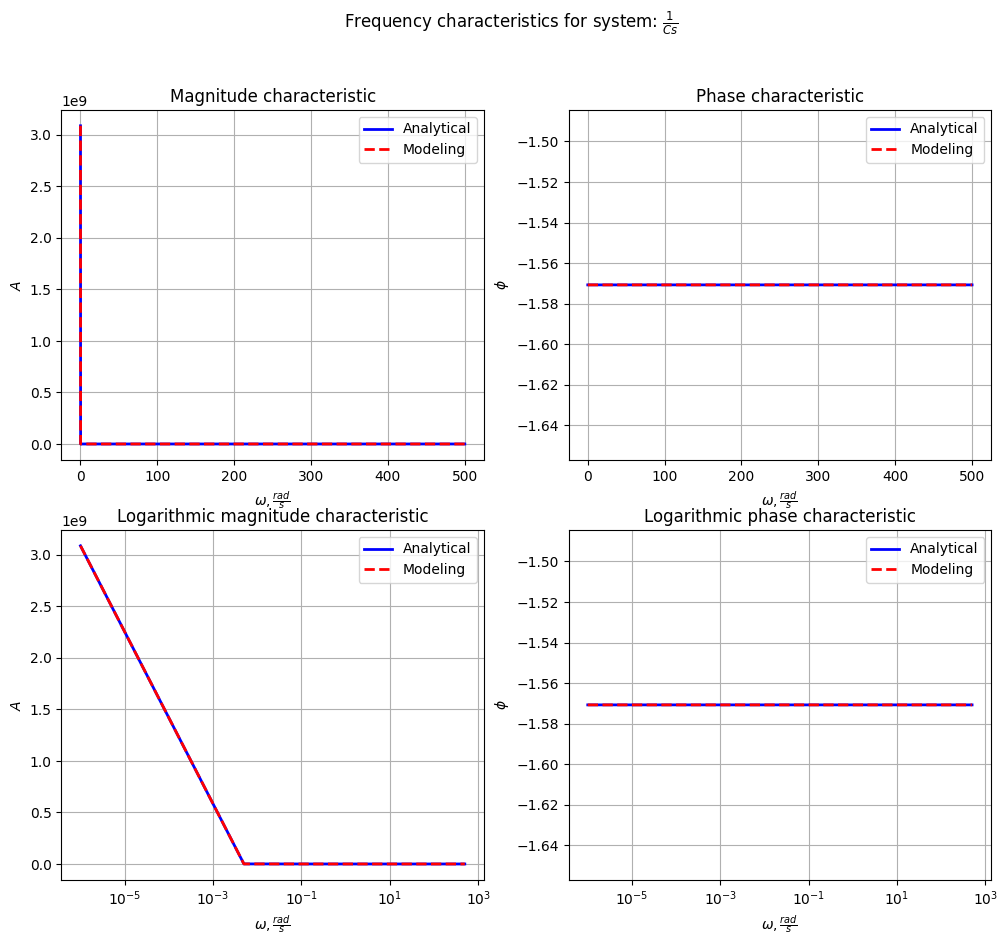
\includegraphics[width=\textwidth]{freq_char_3.png}
    \caption{\label{fig:The-caption-1}Частотные характеристики системы 3 (подвариант 7)}
\end{figure}
\pagebreak

\section{Исследование остальных типовых звеньев}
\subsection*{Brushed DC motor}
\begin{equation}
    J \dot{\omega} = M, M = k_m I, I = \frac{U+\varepsilon_i}{R}, \varepsilon_i=-k_e \omega
\end{equation}
Путем преобразований можем получить дифференциальное уравнение (апериодическое звено первого порядка):
\begin{equation*}
    \dot{\omega} + \frac{k_mk_e}{JR}\omega =\frac{k_m}{RJ}U, W(s)=\frac{k_m}{RJs + k_mk_e}
\end{equation*}
Временные характеристики:
\begin{equation*}
    y_{i.r.}=\mathcal{L}^{-1}(W(s)) = \frac{k_{m} e^{- \frac{k_{e} k_{m} t}{J R}} \theta(t)}{J R}
\end{equation*}
\begin{equation*}
    y_{s.r.}=\mathcal{L}^{-1}(\frac{1}{s}W(s)) = \frac{\theta(t)}{k_{e}} - \frac{e^{- \frac{k_{e} k_{m} t}{J R}} \theta(t)}{k_{e}}
\end{equation*}
Проведем моделирование системы и сравним с аналитически полученным поведением:
\begin{figure}[h]
    \centering
    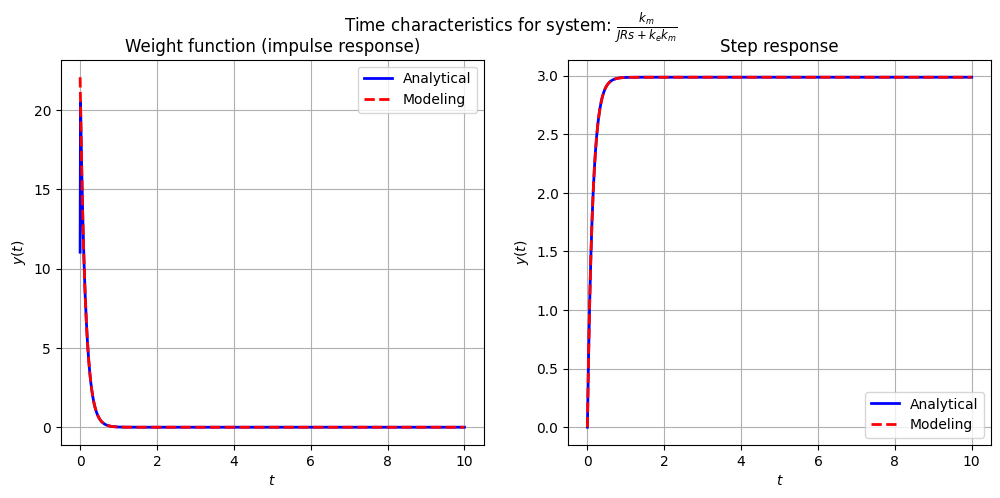
\includegraphics[width=\textwidth]{time_char_1.png}
    \caption{\label{fig:The-caption-1}Временные характеристики системы 1 (подвариант 7)}
\end{figure}

Частотные характеристики:
\begin{equation*}
    |W(j\omega)| = \frac{|{k_{m}}|}{\sqrt{J^{2} R^{2} \omega^{2} + k_{e}^{2} k_{m}^{2}}}
\end{equation*}
\begin{equation*}
    Arg(W(j\omega)) = \operatorname{atan}_{2}{(- \frac{J R k_{m} \omega}{J^{2} R^{2} \omega^{2} + k_{e}^{2} k_{m}^{2}},\frac{k_{e} k_{m}^{2}}{J^{2} R^{2} \omega^{2} + k_{e}^{2} k_{m}^{2}} )}
\end{equation*}
Воспользуемся функцией $\bold{bode}$ для численного моделирования частотных характеристик:
\begin{figure}[]
    \centering
    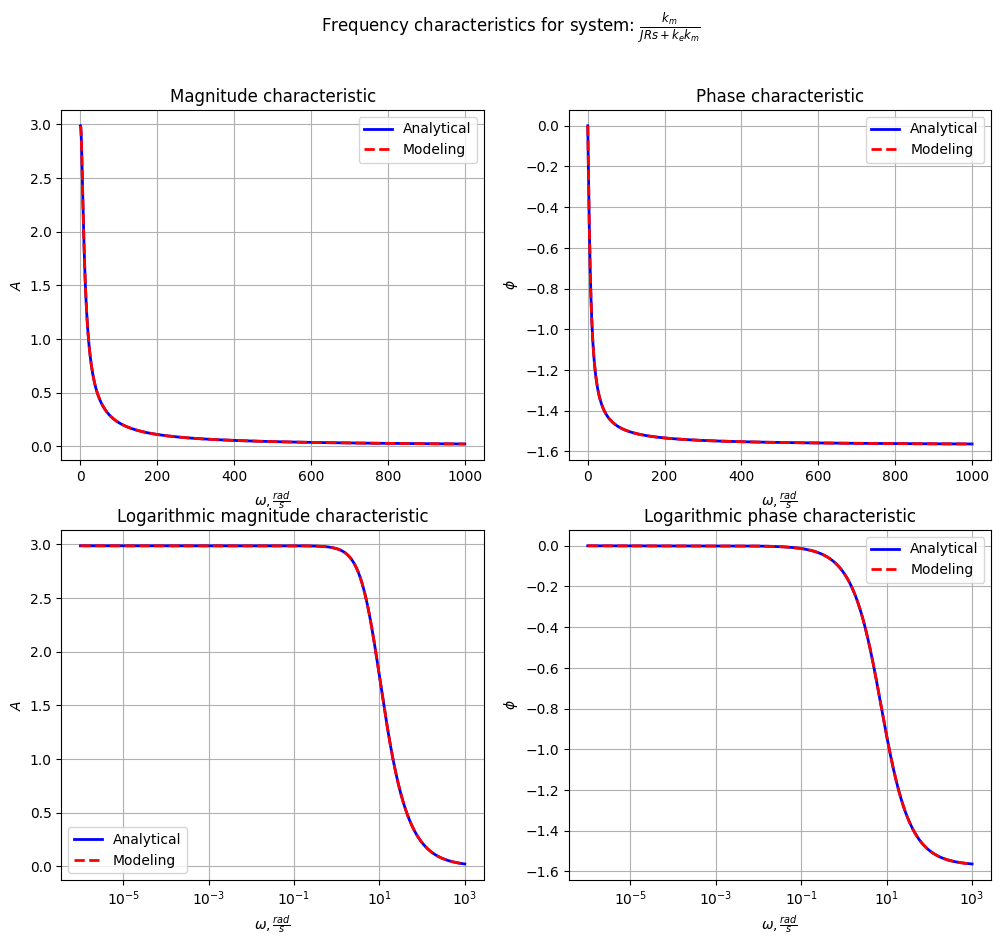
\includegraphics[width=\textwidth]{freq_char_1.png}
    \caption{\label{fig:The-caption-1}Частотные характеристики системы 1 (подвариант 7)}
\end{figure}
\pagebreak

\subsection*{Tachogenerator}
\begin{equation}
    I = \frac{\varepsilon - U_{out}}{R}, \varepsilon = \varepsilon_i + \varepsilon_s, \varepsilon_i=k_e\omega, \varepsilon_s = -L\dot{I}, I = \frac{U_{out}}{R_l}
\end{equation}
Путем преобразований можем получить дифференциальное уравнение (апериодическое звено первого порядка):
\begin{equation*}
    \frac{L}{R_l}\dot{U_{out}} + U_{out}\frac{R_l + R}{R_l} = k_e\omega, W(s) = \frac{\frac{R_lk_e}{L}}{s+\frac{R+R_l}{L}}
\end{equation*}
Временные характеристики:
\begin{equation*}
    y_{i.r.}=\mathcal{L}^{-1}(W(s)) = \frac{R_{l} k_{e} e^{- \frac{t (R + R_{l})}{L}} \theta(t)}{L}
\end{equation*}
\begin{equation*}
    y_{s.r.}=\mathcal{L}^{-1}(\frac{1}{s}W(s)) = \frac{R_{l} k_{e} (e^{\frac{t (R^{2} + 2 R R_{l} + R_{l}^{2})}{L (R + R_{l})}} - 1) e^{- \frac{t (R^{2} + 2 R R_{l} + R_{l}^{2})}{L (R + R_{l})}} \theta(t)}{R + R_{l}}
\end{equation*}
Проведем моделирование системы и сравним с аналитически полученным поведением:
\begin{figure}[h]
    \centering
    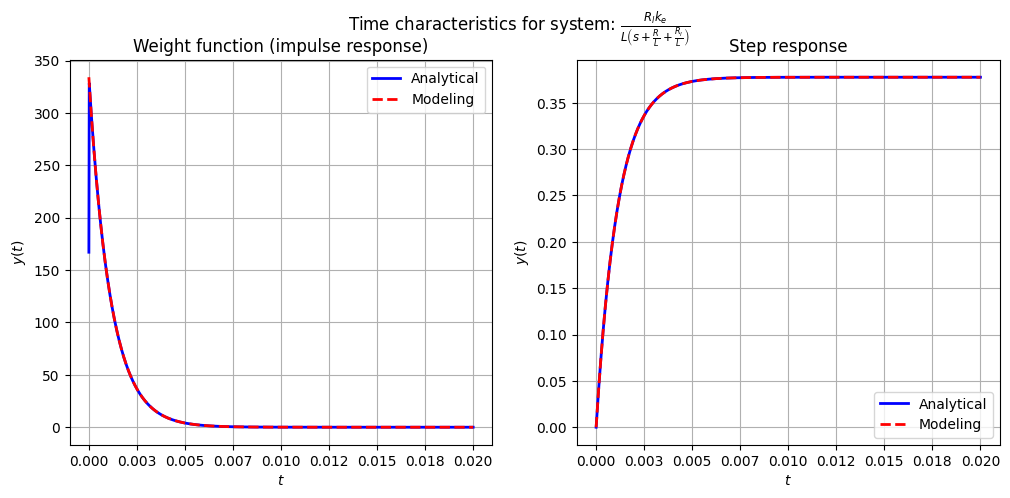
\includegraphics[width=\textwidth]{time_char_4.png}
    \caption{\label{fig:The-caption-1}Временные характеристики системы 4 (подвариант 16)}
\end{figure}

Частотные характеристики:
\begin{equation*}
    |W(j\omega)| = \frac{|{\frac{R_{l} k_{e}}{L}}|}{\sqrt{\frac{L^{2} \omega^{2} + R^{2} + 2 R R_{l} + R_{l}^{2}}{L^{2}}}}
\end{equation*}
\begin{equation*}
    Arg(W(j\omega)) = \operatorname{atan}_{2}{(- \frac{L R_{l} k_{e} \omega}{L^{2} \omega^{2} + (R + R_{l})^{2}},\frac{R_{l} k_{e} (R + R_{l})}{L^{2} \omega^{2} + (R + R_{l})^{2}} )}
\end{equation*}
Воспользуемся функцией $\bold{bode}$ для численного моделирования частотных характеристик:
\begin{figure}[]
    \centering
    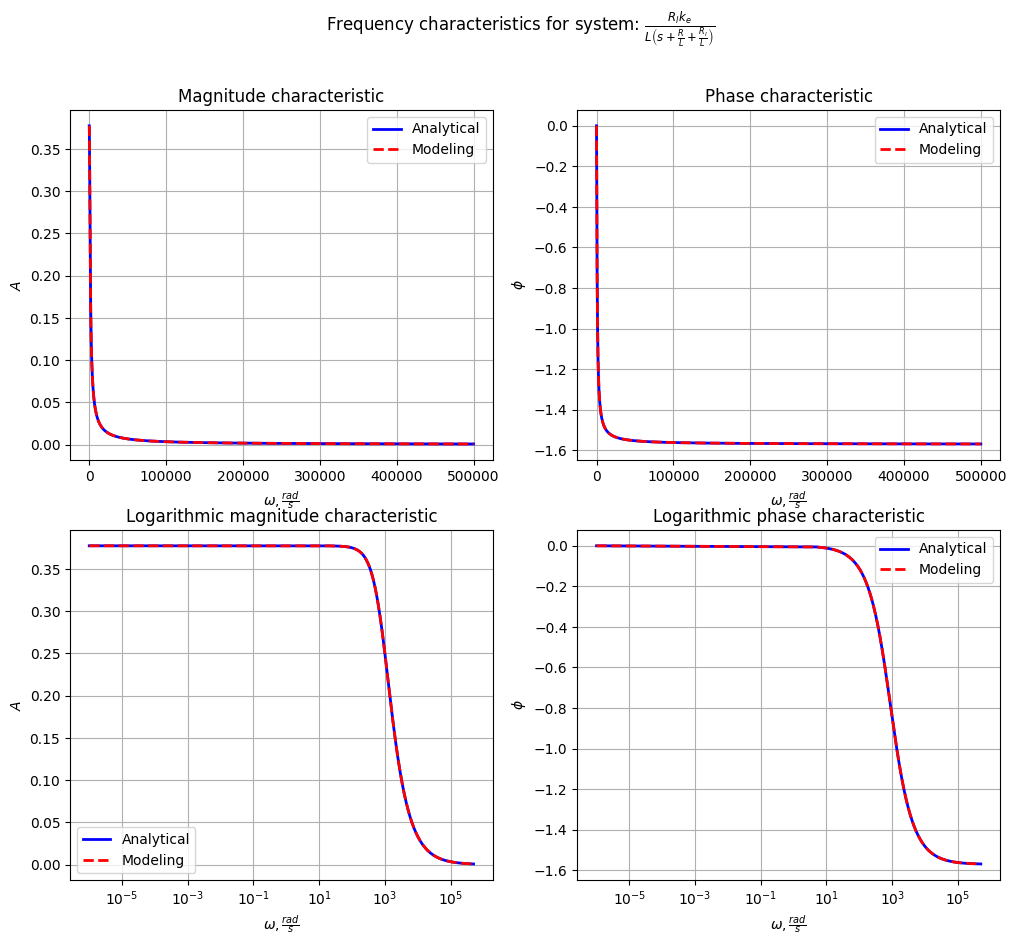
\includegraphics[width=\textwidth]{freq_char_4.png}
    \caption{\label{fig:The-caption-1}Частотные характеристики системы 4 (подвариант 16)}
\end{figure}
\pagebreak

\subsection*{Spring-mass system}
\begin{equation}
    F_{el} = -kx, F=m\ddot{x}, F=F_{ext} + F_{el}
\end{equation}
Путем преобразований можем получить дифференциальное уравнение (колебательное звено):
\begin{equation*}
    m\ddot{x}+kx=F_{ext}, W(s) = \frac{1}{ms^2 + k}
\end{equation*}
Временные характеристики:
\begin{equation*}
    y_{i.r.}=\mathcal{L}^{-1}(W(s)) = \frac{\sin{(t \sqrt{\frac{k}{m}} )} \theta(t)}{m \sqrt{\frac{k}{m}}}
\end{equation*}
\begin{equation*}
    y_{s.r.}=\mathcal{L}^{-1}(\frac{1}{s}W(s)) = \frac{(1 - \cos{(t \sqrt{\frac{k}{m}} )}) \theta(t)}{k}
\end{equation*}
Проведем моделирование системы и сравним с аналитически полученным поведением:
\begin{figure}[h]
    \centering
    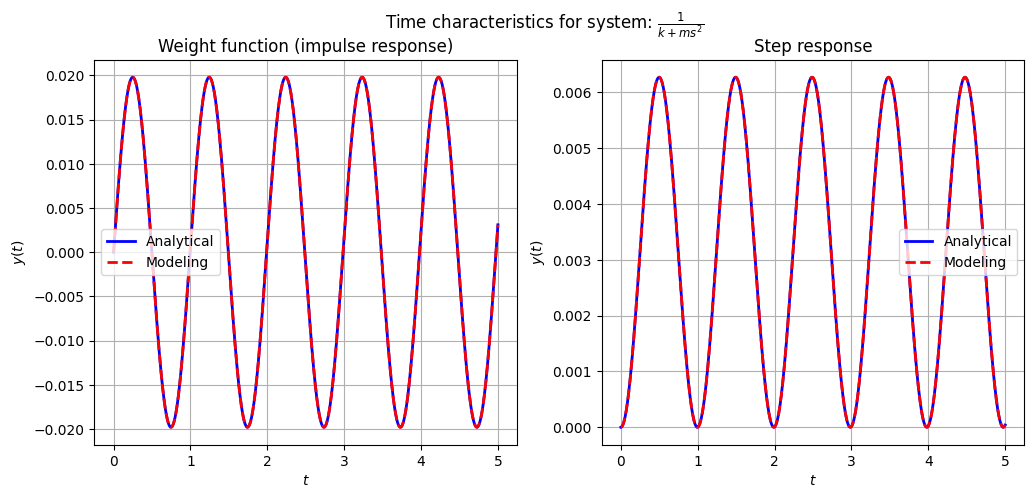
\includegraphics[width=\textwidth]{time_char_5.png}
    \caption{\label{fig:The-caption-1}Временные характеристики системы 5 (подвариант 16)}
\end{figure}

Частотные характеристики:
\begin{equation*}
    |W(j\omega)| = \frac{1}{|{k - m \omega^{2}}|}
\end{equation*}
\begin{equation*}
    Arg(W(j\omega)) = \operatorname{atan}_{2}{(0,\frac{1}{k - m \omega^{2}} )}
\end{equation*}
Воспользуемся функцией $\bold{bode}$ для численного моделирования частотных характеристик:
\begin{figure}[]
    \centering
    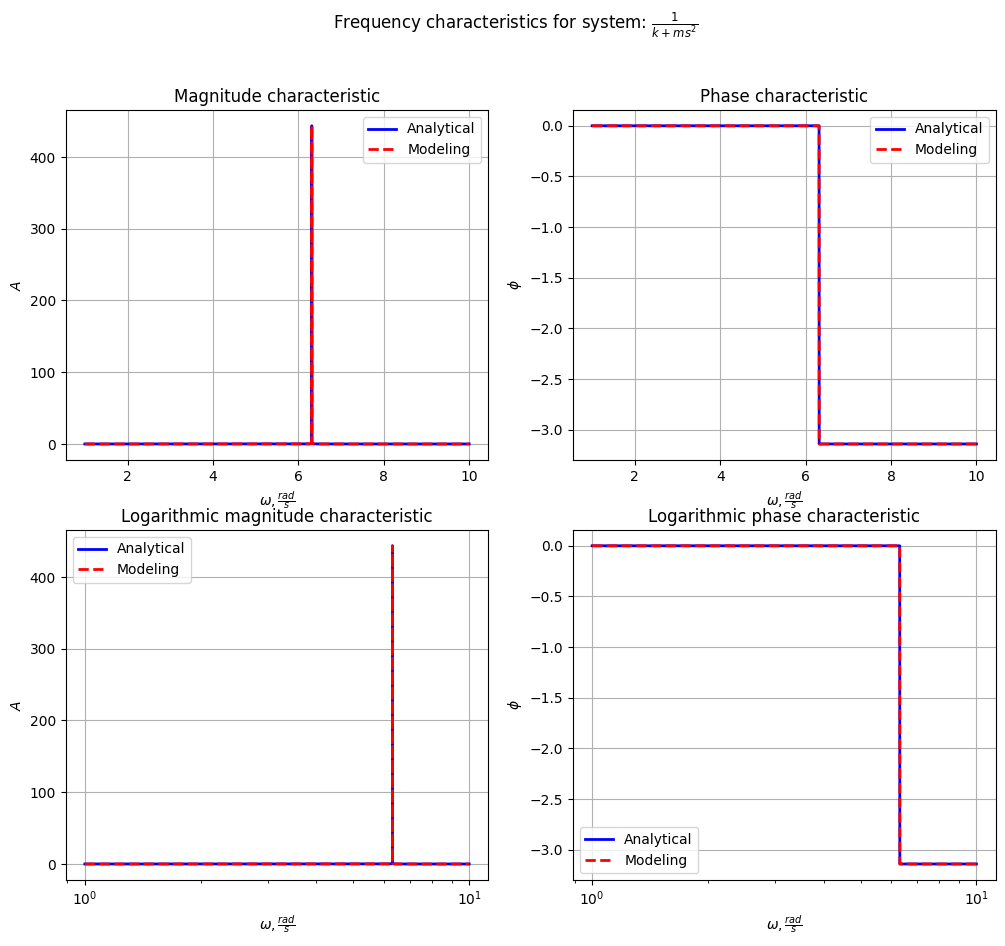
\includegraphics[width=\textwidth]{freq_char_5.png}
    \caption{\label{fig:The-caption-1}Частотные характеристики системы 5 (подвариант 16)}
\end{figure}
\pagebreak

\section{Выводы}
В ходе данной лабораторной работы удалось изучить поведение систем, представляющих собой разные типы динамических звеньев.
\begin{enumerate}
    \item Во всех случаях аналитические результаты подтвердились моделированием.
    \item Поведение систем различных типов динамических звеньев совпало с теоретическими предсказаниями.
\end{enumerate}
\pagebreak